\section{Experimental Results}
\label{sec:evolution-results}

\subsection{RQ1: Types of Changes during KDT Evolution}
\label{sec:evolution-results-rq1}

This research question pertains to the types of changes performed by the testers during \emph{TestSuiteA} evolution. The identified types and their total amount are presented in Table~\ref{table:total_changes}. The first column of the table shows the type of changes as extracted by our change algorithm. The next columns present the total amount of these changes during the \emph{Creation} and \emph{Maintenance} periods (as defined in Section \ref{sec:evolution-introduction-data}) over the 8 months of the study.

\begin{table}
\caption{Types and total amount of changes over the 8-months study}
\label{table:total_changes}
\centering
\begin{tabular}{lrr}
\toprule
change type &  Creation &  Maintenance \\
\midrule
insert documentation          &       \textbf{430} &            2 \\
insert step                   &       135 &           62 \\
insert test case              &        94 &           12 \\
insert user keyword           &       394 &           80 \\
insert variable               &       286 &           77 \\
update documentation       &       106 &           96 \\
update for loop body       &         0 &            0 \\
update for loop condition  &         0 &            0 \\
update name                &        45 &            6 \\
update step                &       249 &          107 \\
update step arguments      &       105 &          \textbf{144} \\
update step expression     &         7 &            6 \\
update step return values  &         0 &            1 \\
update step type           &         5 &            3 \\
update variable definition &        34 &           45 \\
delete documentation       &         0 &            2 \\
delete step                &        25 &           34 \\
delete test case           &        26 &            2 \\
delete user keyword        &        70 &           38 \\
delete variable            &         6 &           23 \\
\midrule
Total                      &      2017 &          738 \\
\bottomrule
\end{tabular}
\end{table}

We see that during \emph{Creation}, the main activities in terms of number of changes is ``insert documentation'', ``insert user keyword'', ``insert variable'' and ``update step''. The first three types of changes are naturally related to test creation, so this outcome is expected. A more interesting finding is that a lot of effort is devoted in documenting the keywords created. After discussing with the QA team, this effort is justified by the fact that this documentation will prove useful in the case of KDT test failures. ``Update step'' refers to modifications of steps of existing keywords. The specific kinds of modifications will be further investigated later in the section (Figure \ref{fig:changes_steps}).
  
\begin{figure}
\centering
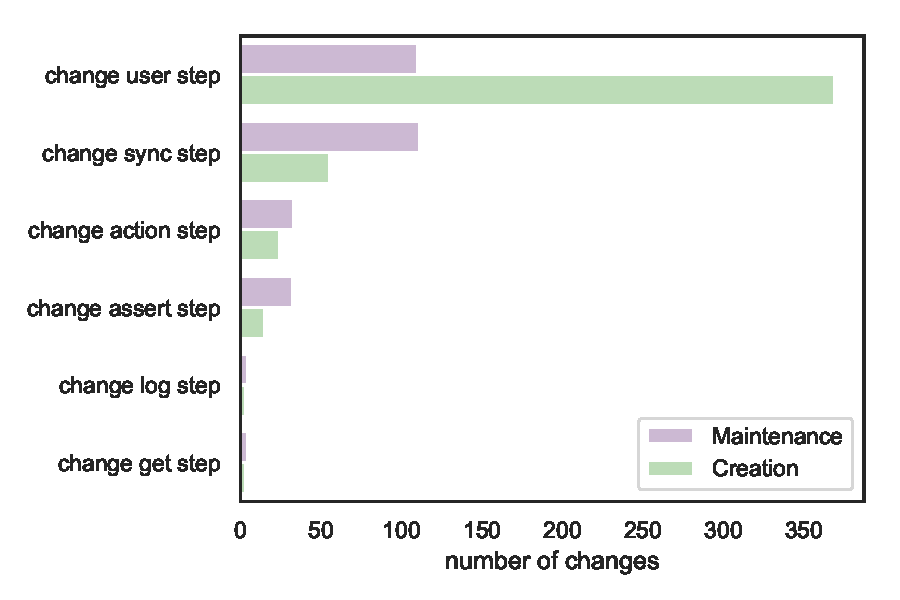
\includegraphics[width=0.7\columnwidth]{figures/evolution/changes_categories.pdf}
\caption{Total number of step changes per type}  
\label{fig:changes_steps}
\end{figure}

During \emph{Maintenance}, the main types of changes performed are the ``update step arguments'', the ``update step'', ``update documentation'' and ``insert user keyword''. After manually analyzing the changes to the arguments, we found two prevalent categories of commonly-changed arguments: arguments referring to \emph{synchronization} between the SUT and the KDT tests, e.g. wait 3 seconds and arguments referring to \emph{locators}, i.e., ways of locating elements in the GUI interface of the SUT. The arguments of the first category are typically used in the \emph{SYNC} category of Table \ref{keywords_categories}, and the latter at keywords of the \emph{ACTION} and \emph{ASSERTION} categories. Our results suggest that keywords belonging to these categories experience a high number of changes. Practitioners corroborate those results and motivate those results in RQ4.

\begin{figure}
\centering
\subfloat[Keyword Level \label{fig:boxplot_depth}]
    {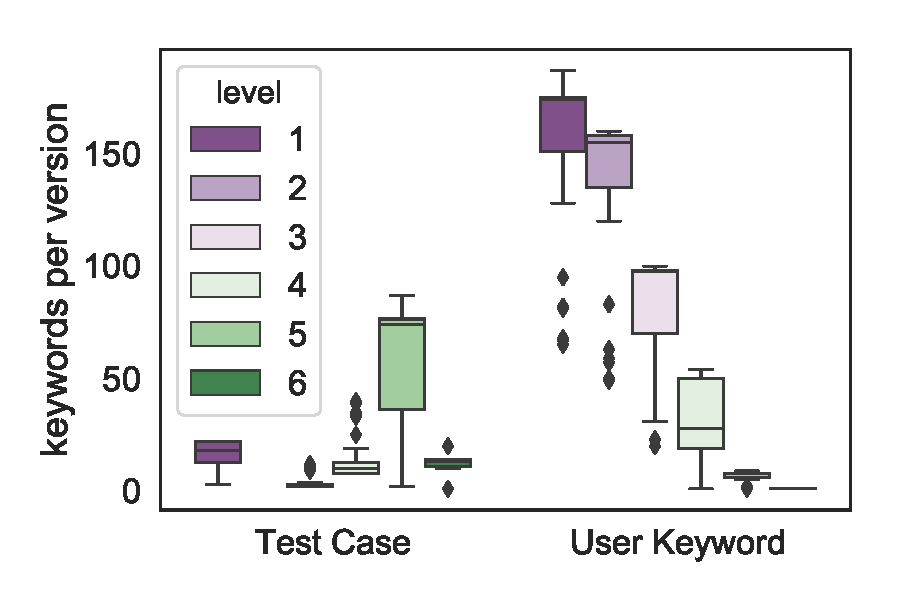
\includegraphics[width=0.45\textwidth]{figures/evolution/boxplot_depth.pdf}}
\subfloat[Keyword Connectivity\label{fig:boxplot_connectivity}]
    {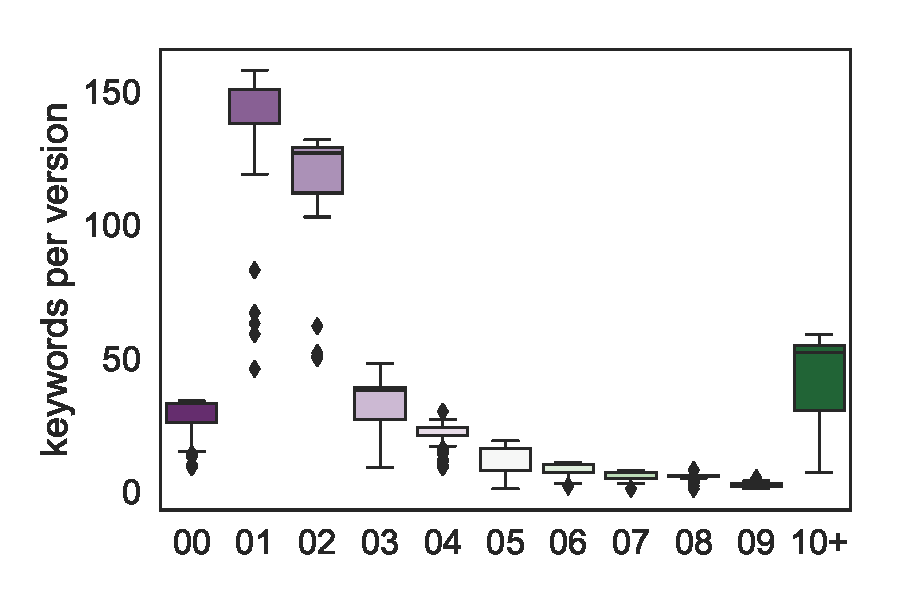
\includegraphics[width=0.45\textwidth]{figures/evolution/boxplot_connectivity.pdf}}\\
\subfloat[Connectivity per level category \label{fig:boxplot_depth_connectivity}]
    {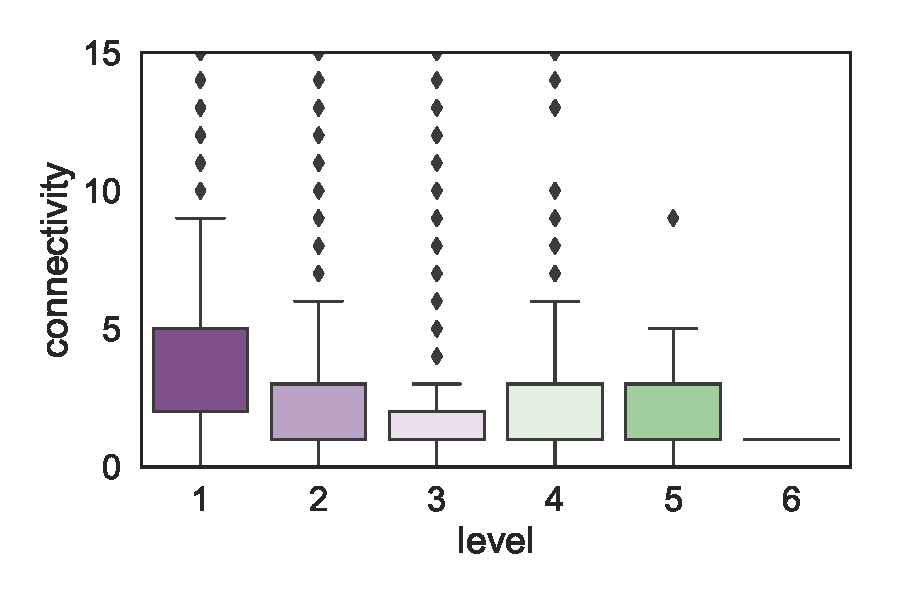
\includegraphics[width=0.45\textwidth]{figures/evolution/boxplot_depth_connectivity.pdf}}
\caption{Understanding KDT Test Suite Complexity}  
\label{fig:code_metrics}
\end{figure}

% susceptible to changes easily. The problem of defining \emph{locators} robust
% to changes has already been explored in the literature
% \cite{leotta_ICST_2015}.

Apart from ``update step arguments'', ``update step'' constitutes one of the most common change for both \emph{Creation} and \emph{Maintenance} periods. To further investigate the nature of these changes, Figure~\ref{fig:changes_steps} plots the number of changes (x-axis) against the category of the enclosing keywords (y-axis), as presented in Table~\ref{keywords_categories} with different colors for the periods studied.

As can be seen from the figure, \emph{change user steps} is by far the greatest activity during creation, we see that changes in \emph{synchronization steps} are equally important during maintenance. The interview conducted in RQ4 motivate that finding and explains it by the fact that many keywords are refactored during creation of new tests to become more generic so they can be reused. Another trend is that except for the \emph{user steps}, all other categories evolve more during maintenance. This is due to the same effect as mentioned earlier where changes in the application cause tests to break. \emph{user steps} are less affected by that effect since they are more abstract and thus less sensitive to trivial application evolution.

\subsection{RQ2: KDT Complexity and Evolution}
\label{sec:evolution-results-rq2}

The results for RQ2 are split into two parts: first, results about the complexity of KDT test suites are reported; and, second, the way this complexity affects its evolution is presented.

\subsubsection{KDT complexity}
\label{sec:kdt-test-suite}

To understand KDT complexity, we calculate the \emph{keyword level} and \emph{connectivity} metrics, defined in Section~\ref{sec:evolution-protocol-definitions}. The first metric refers to the different ``abstraction levels'' (moving from pure technical to requirements expression) of the test suite and the second one, to the reusability among the keywords. Figures \ref{fig:boxplot_depth} and \ref{fig:boxplot_connectivity} present the corresponding results.

Figure~\ref{fig:boxplot_depth} depicts our results of the \emph{keyword level} for \emph{Test Cases} and \emph{User Keywords}, with the y-axis referring to the number of keywords per version. Recall that \emph{Test Cases} are the complete instantiation of a test - root node in the tree representation - and \emph{User Keywords} are user defined abstraction of the steps - intermediate nodes in the tree representation - (see also Section~\ref{sec:introduction-test-scripting}). As can be seen from the figure, most \emph{Tests Cases} are relatively complex, with a level of 5, whereas most \emph{User Keywords} are simple (levels 1 to 2). This indicates that most user defined actions remain simple, in accordance with the philosophy of KDT.

Regarding the keyword reusability, Figure~\ref{fig:boxplot_connectivity} plots the number of keywords per version (y-axis) with the \emph{keyword connectivity} (x-axis). As can be seen, there is a high degree of reusability among \emph{User Keywords}. More precisely, only 20.34\% of the lines of code are used only once. Overall, the reused keywords amount to 51.56\% of the total lines of code of \emph{TestSuiteA}. As we will see next, this reusability is key to the decreased cost of the KDT maintenance.

Another interesting finding is the presence of dead test code, i.e., keywords not used anywhere in \emph{TestSuiteA}; these keywords have a connectivity of 0 in Figure \ref{fig:boxplot_connectivity}. In total, 5.58\% of the keywords were not used, which amounts to 4.58\% of the test code base. When we presented our findings to the QA team, they were surprised and confirmed the existence of dead code, explaining that there is no tooling to support such analysis. Our tool solves this issue and has been integrated into the team's test code development processes (Chapter~\ref{chap:ikora-inspector}).

To investigate whether keywords of a particular level tend to be more reused than others, Figure~\ref{fig:boxplot_depth_connectivity} plots the keyword connectivity among the different keyword levels. By examining the figure, it becomes clear that keywords levels exhibit relatively high connectivity, indicating that the reusability of keywords is not restricted to a particular level with the exception of level 1 showing a slightly higher connectivity.


% Manual analysis showed that this is due to the fact that different \emph{User
% Keywords} were created for different features of the software, therefore
% limiting reusability.

\subsubsection{KDT complexity and evolution}
\label{sec:kdt-complexity-evolution}

The second part of RQ2 refers to the evolution of KDT and how their complexity affects it. To better understand the amount of changes performed during test code evolution, Figure~\ref{fig:churn} presents the test code churn (y-axis) over the eight-month period analyzed (x-axis), with a similar setup to Figure \ref{fig:project_evolution}.

The purple line in the figure denotes the average churn across \emph{TestSuiteA} evolution and the light purple, its variance represented here by the standard deviation. From the figure, it can be observed that during \emph{Creation}, the churn is 8.13\%, on average, whereas in the \emph{Maintenance} period, its value is 3.61\%. Overall, keywords are changed with a churn rate of 5.11\%. This number suggests that keywords are not entirely rewritten, but localized modifications are performed.

\begin{figure}
\centering
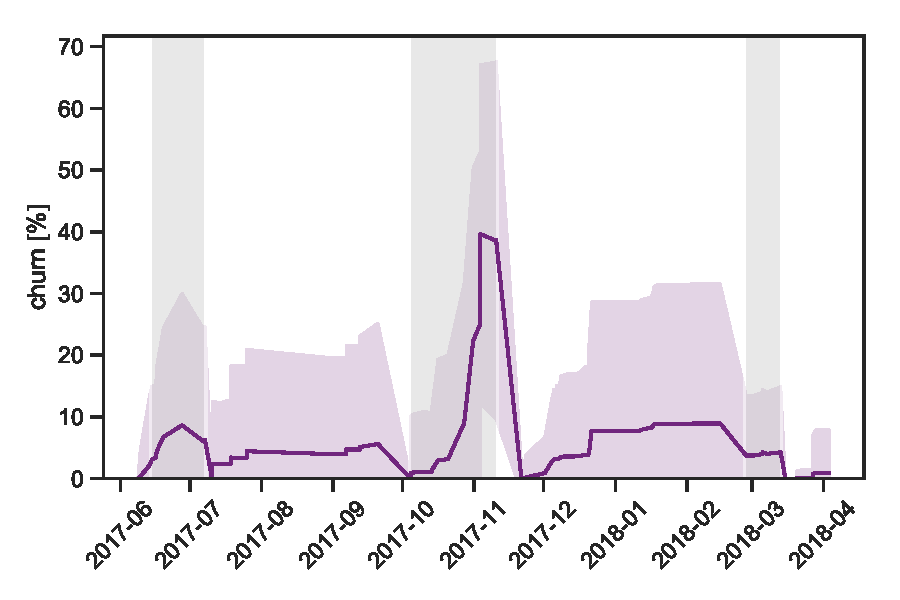
\includegraphics[width=0.7\columnwidth]{figures/evolution/time_series_churn.pdf}
\caption{KDT test code evolution: Churn over time}  
\label{fig:churn}
\end{figure}

To investigate further how the complexity of the KDT test code affects its evolution, Figure~\ref{fig:changes} plots the number of changes, for the whole period studied, against the keyword connectivity and level and Figure~\ref{fig:churn:analysis} plots the churn against the same metrics.

After examining Figure~\ref{fig:changes_connectivity}, it becomes clear that keyword reused one to three times are mostly changed. Keywords with higher connectivity do not change that often. Moreover, the figure shows that changes are performed on dead code (connectivity 0). This confirms that testers are unware of the fact that these keywords are never executed, generating easy to avoid maintenance. Regarding the results for changes and level, depicted in Figure~\ref{fig:changes_depth}, we can observe that the changes to \emph{Test Cases} do not follow a specific trend, whereas for the changes to the \emph{Users Keywords}, the lower level the keyword is, the more it is suceptible to be changed.

\begin{figure}
\centering
\subfloat[Connectivity \label{fig:changes_connectivity}]{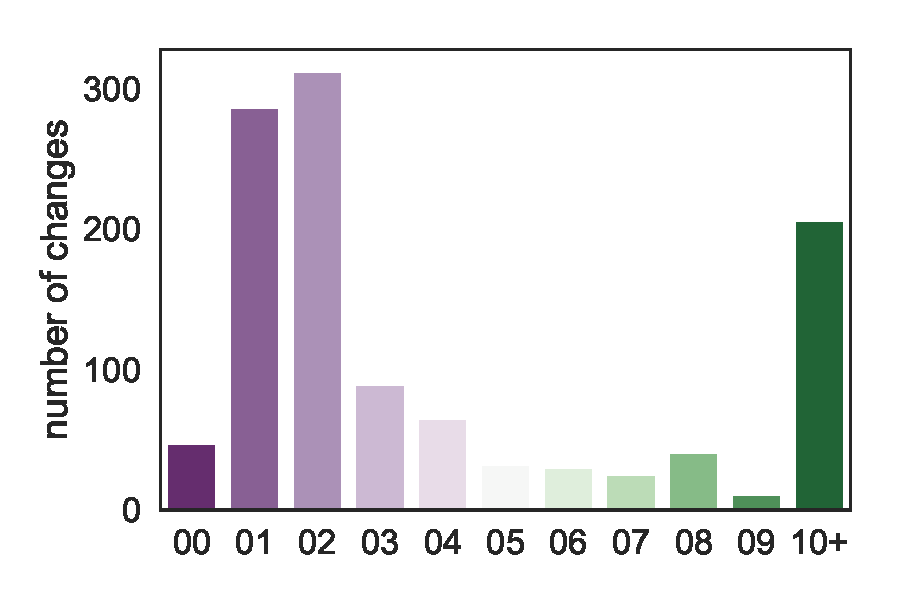
\includegraphics[width=0.45\textwidth]{figures/evolution/changes_connectivity_class_total.pdf}}
\subfloat[Level \label{fig:changes_depth}]{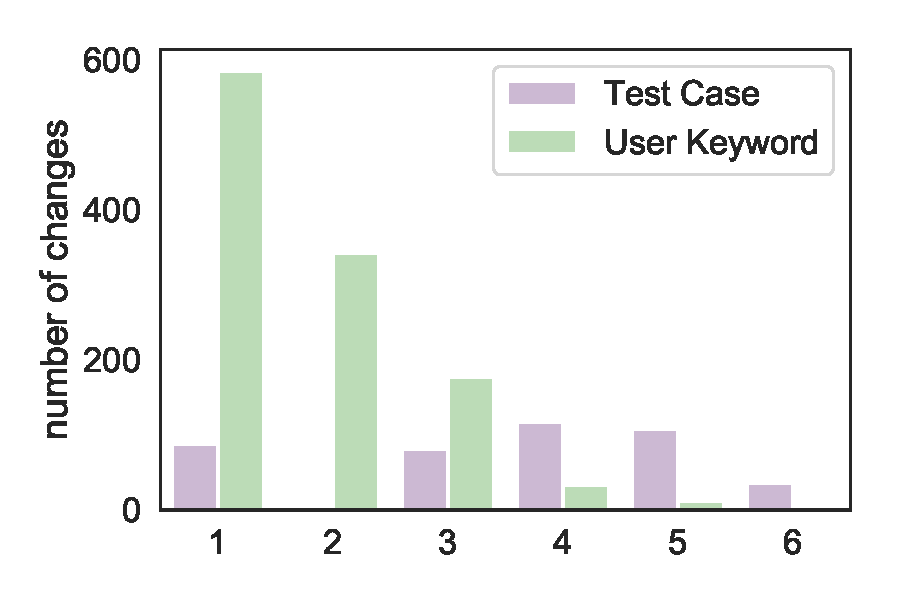
\includegraphics[width=0.45\textwidth]{figures/evolution/changes_depth_total.pdf}}
\caption{Changes distribution according to level and connectivity}  
\label{fig:changes}
\end{figure}

\begin{figure}
\centering
\subfloat[Connectivity \label{fig:churn_connectivity}]{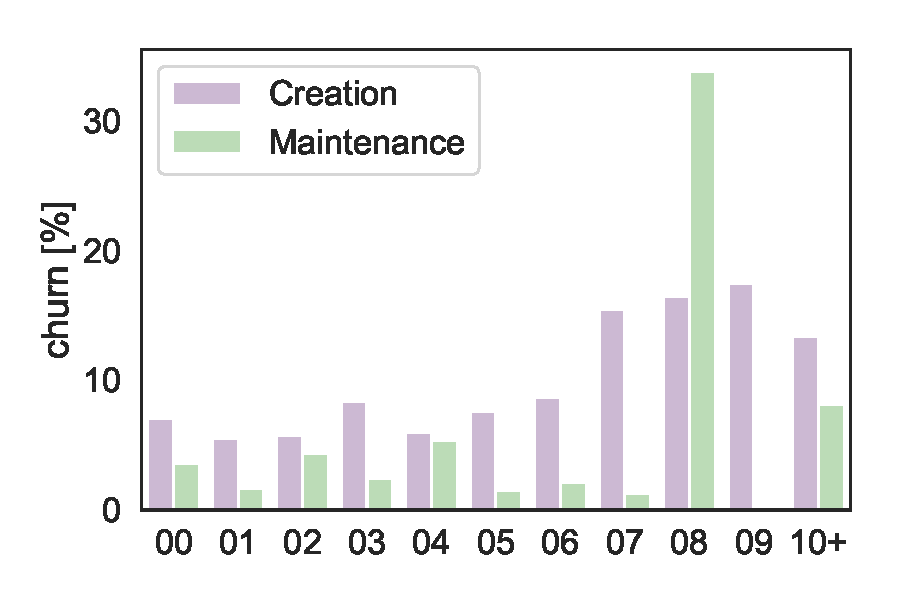
\includegraphics[width=0.45\textwidth]{figures/evolution/barplot_connectivity_class_churn.pdf}}
\subfloat[Level \label{fig:churn_depth}]{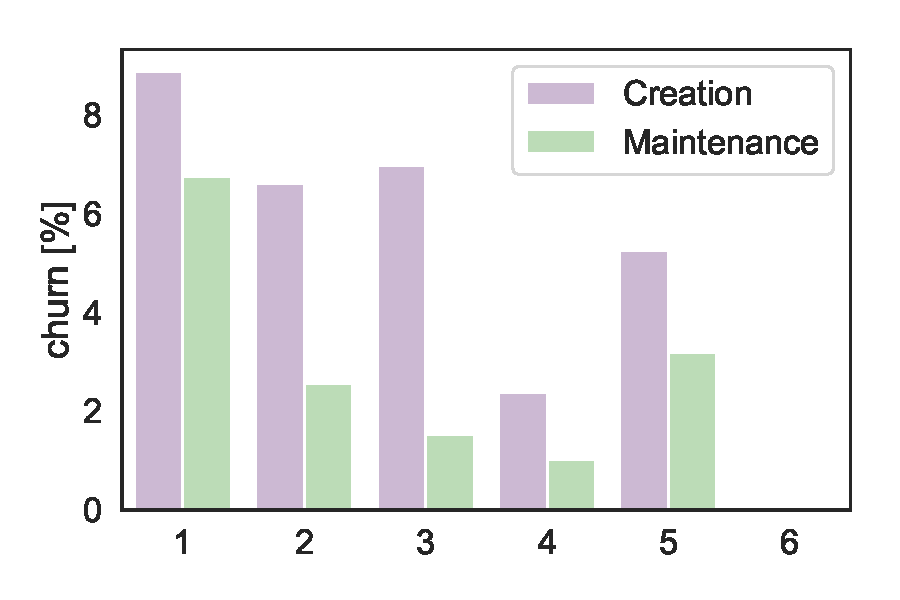
\includegraphics[width=0.45\textwidth]{figures/evolution/barplot_depth_churn.pdf}}
\caption{Churn distribution according to level and connectivity}  
\label{fig:churn:analysis}
\end{figure}

Regarding our findings on the relation between churn rate and connectivity, depicted in Figure~\ref{fig:churn_connectivity} for the \emph{Creation} and \emph{Maintenance periods}, we can conclude that, during \emph{Creation}, keywords that are reused often, i.e. higher connectivity, exhibit approximately 50\%-60\% increased churn rate, whereas, during \emph{Maintenance} the opposite holds. Finally, regarding the results presented in Figure~\ref{fig:churn_depth} about churn and keyword level, we can see that, during \emph{Creation}, keywords with lower levels exhibit high churn values, whereas in \emph{Maintenance} this only holds for keywords of level 1. These results suggest that low level, highly reused keywords (basic action on the SUT), are evolving at a higher rate.

As we saw earlier, in \emph{TestSuiteA} evolution, keyword changed with a churn rate of 5.11\% but we also saw in the previous section that keywords are reused often. This raises the questions: How many changes have been saved due to the reusability of the keywords? To answer this question, we compare the the number of changes applied to \emph{TestSuiteA} to the same suite without the keyword abstraction as explained in Section~\ref{sec:evolution-protocol-rq2}. We find that using KDT reduces the number of changes applied on \emph{TestSuiteA} by 70.77\% during ``Creation'', by 72.69\% during ``Maintenance'' with an overall reduction during the entire period of 71.31\%. 

\subsection{RQ3: KDT, Test Clones and Evolution}
\label{sec:evolution-results-rq3}

In RQ3, we explore whether KDT test suites contain test clones and how these clones affect \emph{TestSuiteA} evolution. Table~\ref{table:co_evolution} presents the corresponding results. The table presents the total number of keywords that appear during the evolution of \emph{TestSuiteA} (for all 129 versions) for each type of clone detected (first column -- Type I keyword clones, Type II and non-clones(``Others'')) and each type of evolution (second column). The types of evolution studied are divided into three categories: keywords that are evolving strictly in the same way as others (``Co-evolution''), keywords that are evolving independently from others (``Evolution'') and keywords that do not evolve (``No change'').

We can observe several interesting findings from the table. First, we see that Type I and Type II clones comprise 30.2\% of the total amount keywords, indicating that almost one third of the test code written is duplicated. This finding highlights the fact that practitioners applying KDT will benefit from tools and techniques that can assist them in managing test clones.

Secondly, our results suggest that approximately 50\% of the Type I test clones evolve in the exact same way, indicating that the practitioners apply the same changes multiple times, wasting valuable effort. This is a high figure, especially when compared to the co-evolution of non-cloned keywords which is 4.9\%. Taking these results into consideration and the fact that almost 10\% of the keywords are evolving in the same way, it becomes obvious that automated refactoring techniques can reduce the maintenance effort of KDT test suite evolution.

\begin{table}
\caption{KDT Test Clones and Evolution}
\label{table:co_evolution}
\centering
\begin{tabular}{l|rrr|r}
  \toprule
         & \multicolumn{3}{c|}{Types of Evolution}                  \\
Keywords & Co-evolution &  Evolution &  No change &  Total          \\
\midrule
Type I  &          3526 &       3599 &        412 &   7537 (13.7\%) \\
Type II &           171 &       8462 &        491 &   9124 (16.5\%) \\  
Others  &          1888 &      33433 &       3184 &  38505 (69.8\%) \\
\midrule                                   
Total   &          5585 &      45494 &       4087 &  55166 (100\%)  \\ 
Percent &        10.1\% &     82.5\% &      7.4\% &    -            \\
\bottomrule
\end{tabular}
\end{table}

Finally, another interesting result exhibited in Table~\ref{table:co_evolution} concerns the overall evolution. We observe that only 7.4\% of the keywords are not evolving. This shows that during the TestSuiteA's evolution more than 90\% of the keywords are modified.

\subsection{RQ4: Benefits and challenges of KDT: The Practitioners' perspective}
\label{sec:evolution-results-rq4}

This research question pertains to the benefits and challenges of KDT as perceived by the practitioners. In the following, we present the main findings of our interviews grouped by the two main questions of our study:

\subsubsection{What are the benefits and challenges of adopting KDT?}

All interviewees agreed on two main benefits of KDT: the low learning curve and its simple syntax. Thanks to its syntax that is close to the natural language, new users can easily start being productive.  This syntax is also well-suited for communication purposes with teams that may have different backgrounds and expertise. The layered structure of keywords (i.e. the different keyword levels) plays an important role in facilitating this by hiding the technical details at the lower levels of the test suite and exhibiting the more business-oriented at the higher levels.

The main challenges encountered by the practitioners reside in their interaction with the SUT. Even a small evolution of the SUT can easily break the tests. Additionally, the testers discuss that finding the elements of the SUT that will be used in the tests is challenging, especially in applications where testability was not the primary concern.

\subsubsection{What kind of changes are performed on the test suite and why?}

The testers report two main reasons for the changes: SUT evolution and keyword adaptation.

Regarding the SUT evolution, the testers reported that as the SUT evolves, its components evolve as well which will cause the tests to adapt. The testers focus on two types of changes that are in according to our findings regarding RQ1 (cf. Section \ref{sec:evolution-results-rq1}): \emph{locators}, i.e., finding which GUI elements of the SUT should be used in the tests and \emph{synchronization} issues between the tests and the SUT.

Regarding keyword adaptation, the testers said that they create keywords in a ``best effort'' approach to cover the current needs. As new features of tests are developed, keywords are modified to become more generic. This fact explains the results illustrated in Figure~\ref{fig:changes_steps} where we observed many changes in \emph{user steps} during \emph{Creation}.